\documentclass[12pt,a4paper]{article}
\usepackage[top=2.7cm, bottom=2cm, left=2cm, right=2cm]{geometry}
\usepackage[utf8]{inputenc}
\usepackage{CJKutf8}
\usepackage{enumitem}
\usepackage{verbatim}


%% Useful packages
\usepackage{amsmath,amssymb}
% \usepackage{subfigure}
\usepackage{graphicx,wrapfig}
\usepackage[dvipsnames,table]{xcolor}
\usepackage[table]{xcolor}
\usepackage{url}
\usepackage{setspace}
\usepackage[colorlinks=true,anchorcolor=black,linkcolor=Blue,urlcolor=RoyalBlue]{hyperref}
\usepackage[linesnumbered,ruled,vlined]{algorithm2e}
\usepackage{threeparttable}

\usepackage{tikz}
\usepackage{blindtext}
\usepackage{titlesec}
\usepackage{courier}
\usepackage{pdfpages}

\usepackage{lastpage}
\usepackage{fancyhdr}
\setlength{\headheight}{0pt}
\renewcommand{\headrulewidth}{1pt} % remove lines
\renewcommand{\footrulewidth}{0pt}
\pagestyle{fancyplain}
\fancyhf{}
\lhead{
  \textcolor{Gray}{Group 2}
}
\rhead{
  \begin{CJK}{UTF8}{bkai}
  \textcolor{Gray}{實驗物理學實驗結報}
  \end{CJK}
}
\lfoot{
   \textcolor{Gray}{March 20}
  }
\rfoot{
  \thepage/\pageref{LastPage}
  }

\title{\vspace{-0.5cm}
       {\bf \textcolor{black}{{\LARGE 
       \begin{CJK}{UTF8}{bkai}
       實驗物理學(二)\\
       \vspace{6pt}
       實驗結報\\
       \vspace{60pt}
       實驗三、運算放大器\\
       \vspace{6pt}
       Operational Amplifier
       \end{CJK}
       }}
       }
       }
\author{}
\date{}

\begin{document}
\begin{CJK}{UTF8}{bkai}

\maketitle
\thispagestyle{empty}

\vspace{10cm}
\begin{center}
{\large 第二組}\\ \vspace{12pt}
{\large \makebox[3em][s]{洪\hspace{\fill}瑜} B125090009}\\ \vspace{6pt}
{\large \makebox[3em][s]{黃巧涵}  B122030003}\\ \vspace{6pt}
{\large \makebox[3em][s]{洪懌平} B102030019}\\ \vspace{12pt}
{\large 2025/05/20}\\
\end{center}

\clearpage

\vspace{1cm}
\begin{center}
{\large\bf\sc 摘要}
\end{center}

\noindent 

此次實驗研究主題為運算放大器(型號:UA741) ,使用電源供應器、訊號產生器及麵包板等器材搭建反相放大器(Inverting Amplifier)、同相放大器(Non-inverting Amplifier)及隨耦器(Voltage Follower, Buffer Amplifier),並以示波器紀錄經運算放大器產生之波型。 

\section{前言}
\hfill

本實驗的主要目標是探討運算放大器的基本應用,我們將透過實驗驗證反相放大器(Inverting Amplifier)、同相放大器(Non-inverting Amplifier)及隨耦器(Voltage Follower, Buffer Amplifier)的特性與行為。 

In the following subsections, we will introduce the principles utilized in these experiments.

\subsection{運算放大器 (Operational Amplifier or Op-Amp)}
\hfill

是一種電子元件,主要用於放大輸入訊號。它有極高的增益(gain),可以將微弱的電 壓訊號放大到所需的水平。運典型的運算放大器電路有兩個輸入端(反相輸入端−和非反相輸入端+)以及一個輸出端。可以利用外接電阻或電容的方式使放大器有不同的形式,如同相放大器、反相放大器、比較器及電壓跟隨器等等。 

\begin{figure}[h]
    \centering
    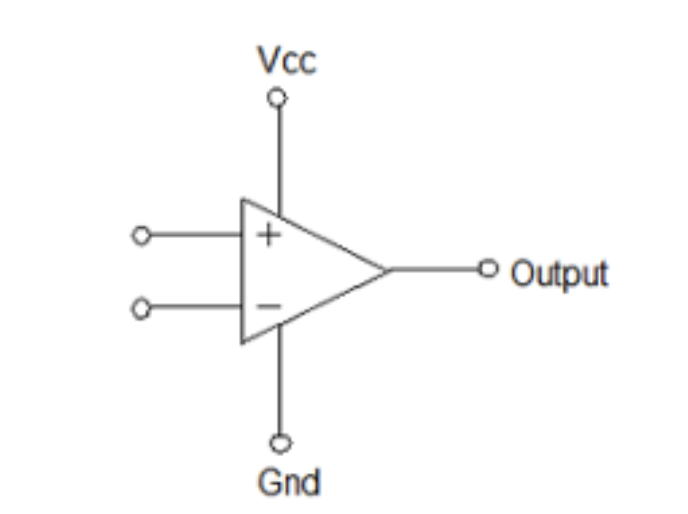
\includegraphics[width=0.5\linewidth]{figures/opamp.png}
    \caption{運算放大器電路示意圖}
    \label{fig:opamp}
\end{figure}

Fig.\ref{fig:opamp}為放大器的簡易連接,運算放大器會將兩個輸入端之電壓差值乘以其增益量,而因增益量很高,需在輸出到輸入間連接電阻降低增益。 

\subsection{非反相放大器}
\hfill

Fig.\ref{fig:noninvert}為同相放大器之電路,此為非反相輸入接收訊號,而反相輸入連接在 $R_2$和$R_1$之間。當輸入訊號為正或負移動時,輸出會保持同相,並保持反相輸入端的電壓與同相輸入端之電壓相同。


\begin{figure}[h]
    \centering
    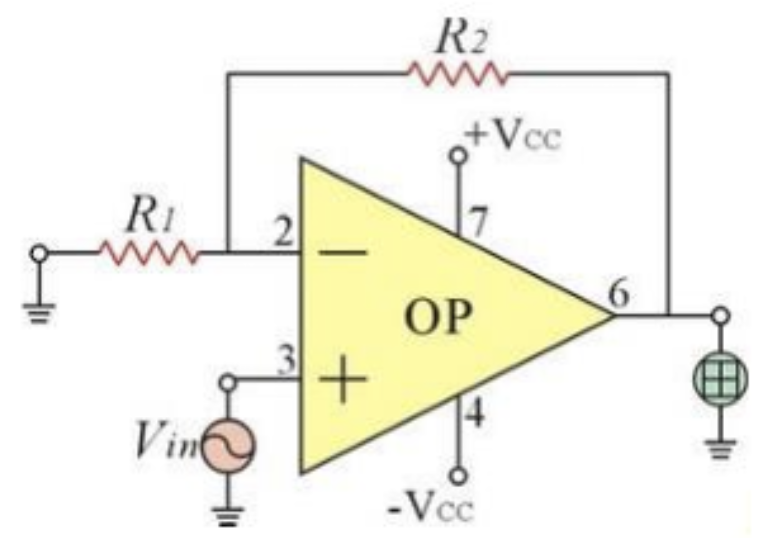
\includegraphics[width=0.4\linewidth]{figures/noninvert.png}
    \caption{同向放大器電路示意圖}
    \label{fig:noninvert}
\end{figure}

本實驗之結構概念:
\begin{enumerate}
    \item 輸入電壓($V_{in}$)連接到非反相輸入端(標記為+端),即第3腳
    \item 反相輸入端(標記為-端,腳位2)通過電$R_1$接地,並透過電阻$R_2$與輸出$V_{out}$連接(第6腳)
\end{enumerate}

公式推導:
\begin{itemize}
    \item 由於運算放大器的增益非常高,並且電路中使用了負回授,根據「虛短」的特性,可以認為反相$V_-$的電壓接近於非反相端的電壓。因此
    \begin{equation}
        V_-\approx V_+ = V_{in}
    \end{equation}
    根據電壓分壓原理,得
    \begin{equation}
        V_-=V_{in}=\frac{R_1}{R_1+R_2}V_{out}
    \end{equation}
    i.e.,
    \begin{equation}
    \label{eq:noninvert}
        V_{out} = V_{in}\left(1+\frac{R_2}{R_1}\right)
    \end{equation}
    \item 增益定義:
    \begin{equation}
        A=\frac{V_{out}}{V_{in}}
    \end{equation}
    再承Eq.\ref{eq:noninvert},得:
    \begin{equation}
        A=1+\frac{R_2}{R_1}
    \end{equation}
\end{itemize}

\subsection{反相放大器}
\hfill

Fig.\ref{fig:invert}為反相放大器之電路,由$R_1$輸入訊號,$R_2$將輸出返回到反相輸入;而若輸入訊號為正,輸出訊號為負,反之亦然。輸出相對於輸入之電壓變化取決於電阻$R_1$和$R_2$的比率。 

\begin{figure}[h]
    \centering
    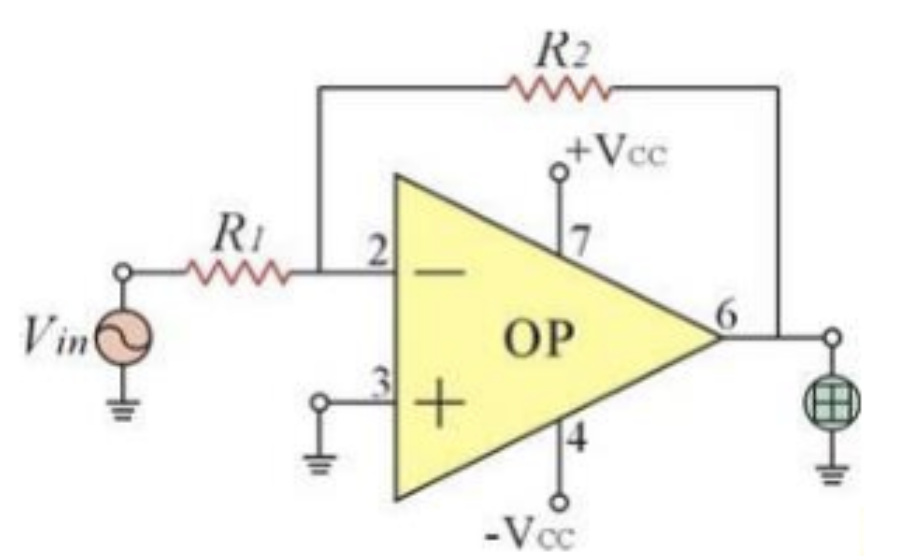
\includegraphics[width=0.5\linewidth]{figures/invert.png}
    \caption{反向放大器電路示意圖}
    \label{fig:invert}
\end{figure}


本實驗之結構概念:
\begin{enumerate}
    \item 輸入電壓($V_{in}$)經過電阻$R_1$接到反相輸入端(標記為-端,即第2腳)
    \item 非反相輸入端(標記為+端,腳位3)接地
    \item 反相輸入端透過電阻$R_2$與輸出端$V_{out}$相連(第6腳)
\end{enumerate}
% \clearpage
公式推導:
\begin{itemize}
    \item 由於運算放大器的增益非常高,並且電路中使用了負回授,根據「虛短」的特性,運算放大器會自動調整輸出電壓,使得反相輸入端的電壓
    \begin{equation}
        V_-\approx V_+ =0
    \end{equation}
    因為$V_+$接地。由於理想運算放大器的輸入阻抗無窮大,所以反相輸入端$V_-$節點的輸入電流可以忽略不計,因此流經$R_1$的電流$I_1$會等於$R_2$的電流$I_2$,使用柯希荷夫電路定律寫出以下表達式:
    \begin{equation}
        \frac{V_{-}-V_{in}}{R_1} = \frac{V_{out}}{R_{2}}
    \end{equation}
    i.e.,
    \begin{equation}
        \frac{V_{in}}{R_1} = -\frac{V_{out}}{R_2}
    \end{equation}
    得出$V_{out}$:
    \begin{equation}
    \label{eq:invert}
        V_{out} = -V_{in}\frac{R_2}{R_1}
    \end{equation}
    
    \item 增益定義:
    \begin{equation}
        A=\frac{V_{out}}{V_{in}}
    \end{equation}
    再承Eq.\ref{eq:invert},得:
    \begin{equation}
        A=1+\frac{R_2}{R_1}
    \end{equation}
\end{itemize}

\subsection{隨耦器}
\hfill

\begin{figure}[h]
    \centering
    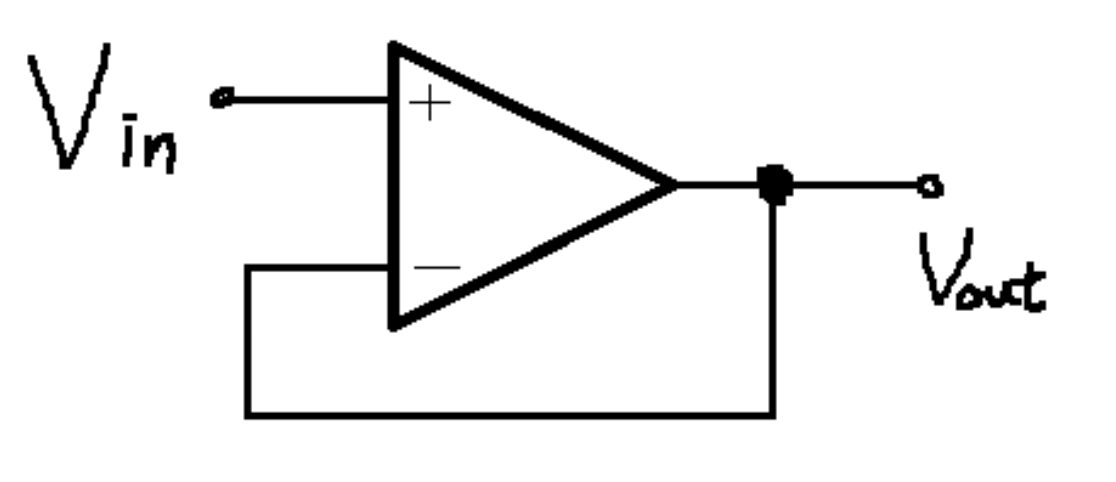
\includegraphics[width=0.5\linewidth]{figures/follower.png}
    \caption{隨耦器電路示意圖}
    \label{fig:follower}
\end{figure}

Fig.\ref{fig:follower}為隨耦器之簡易電路圖,其為一種增益接近1,但具有高輸入阻抗和低輸出阻抗的放大電路;緩衝放大器的輸入與輸出訊號波形相似,但可能會有輕微的相移,主要由於頻率響應、內部電容與寄生電容效應影響。這些因素在高頻時會導致輸出訊號相較輸入訊號略微滯後。


\clearpage

\section{反相放大器}

\subsection{實驗步驟}\label{subsec:step_1}
\begin{enumerate}
    \item 連接電路
    \item 調整訊號產生器參數:$V_{in}$ 使用 1kHz、DC Offset = 0、震幅:0.1V之正弦波;並將其連接接好的電路,使用示波器測量其$V_{out}$。
    \item 將$V_{in}$往上調整,觀察$V_{out}$之震幅最大可達到多少
    \item 改變$V_{in}$頻率,觀察其在高頻與低頻的運作
    \item 將訊號改成三角波輸入並觀察其圖形
    \item 紀錄放大器的輸入阻抗和其增益
\end{enumerate}

\subsection{實驗分析}
\hfill

\begin{enumerate}
    \item $V_{in}$ 用$1KHz$,$DC\ Offset=0$,振幅 $0.1Volt$之弦波輸入,測$V_{out}$,得出電壓增益。

    實際使用$R_1=0.99k\Omega$、$R_2=9.80k\Omega$

\begin{figure}[h]
    \centering
    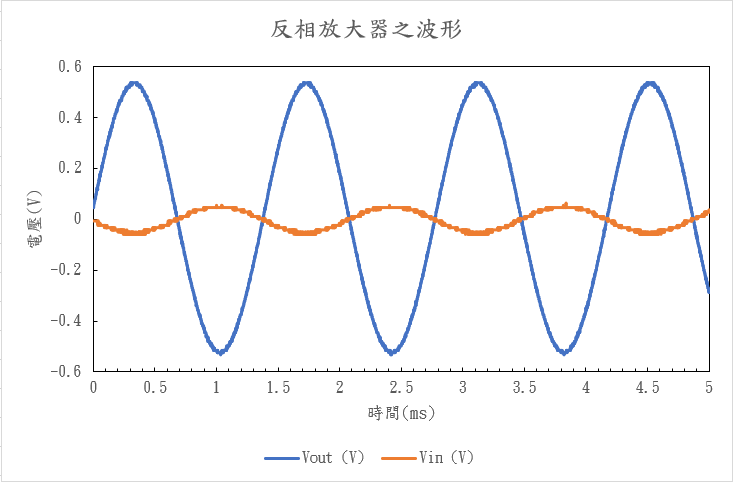
\includegraphics[width=0.7\linewidth]{figures/ia/Inverting amplifier.png}
    \caption{經由反相放大器的輸出波形與原訊號的比較}
    \label{fig:IA_normal}
\end{figure}

輸入振幅:$0.088V$

輸出振幅:$1.043V$

\noindent 分析:

透過Fig.\ref{fig:IA_normal}可見輸入訊號經流放大器後振幅變大,且相位改變$180^\circ$,符合反相放大器的理論特性。而其增益為:$\frac{R_2}{R_1}=\frac{1.04}{0.09} \approx 11.9$,與預期的$\frac{9.80k\Omega}{0.99k\Omega}\approx9.90$,誤差為$20.2\%$。雖然誤差$20.2\%$看似有點大,但我們推測是因為數值較小,導致些微差距就會對誤差計算造成很大的貢獻;單看數值我們認為還在可接受範圍內。

    \clearpage
    
    \item 將$V_{in}$之振幅加大,注意觀察$V_{out}$,$V_{out}$,的最大振幅為多少(不被削截)?

\begin{figure}[h]
    \centering
    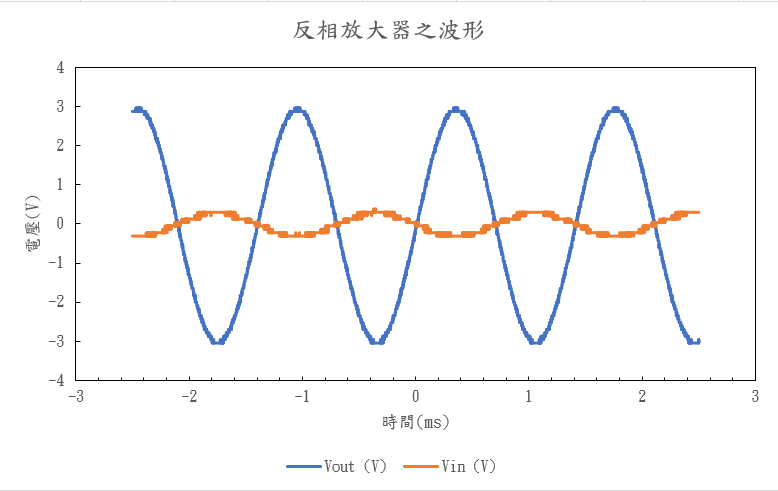
\includegraphics[width=0.7\linewidth]{figures/ia/Maximum output swing of an inverting amplifier.png}
    \caption{反相放大器可測量到的最大振幅}
    \label{fig:IA_Max}
\end{figure}

輸入最大振幅:$0.608V$

輸出最大振幅:$5.879V$

\noindent 分析:

當我們將輸入振幅調整到$0.608V$後觀察到輸出波形產生了削截的情況,可得出反相放大器可放大到的最大振幅為$5.879V$;值得一提的是我們有觀測到削截的現象是先從負端削截,進一步增大輸入振幅後才會看到正端也有削截的情況,我們推測是因為反相放大器會造成相位反轉,所以當振幅往正向變大時,對於輸出端而言是往負電壓的方向加大,所以負端會先碰到最大電壓,導致先觀察到削截的現象;而這個情況下增益為:$\frac{5.88}{0.61}\approx9.64$與理論的$9.90$誤差為$2.6\%$。
    
    \item 改變$V_{in}$的頻率,在很高或很低的頻率此放大器還正常工作嗎?

\begin{figure}[h]
    \centering
    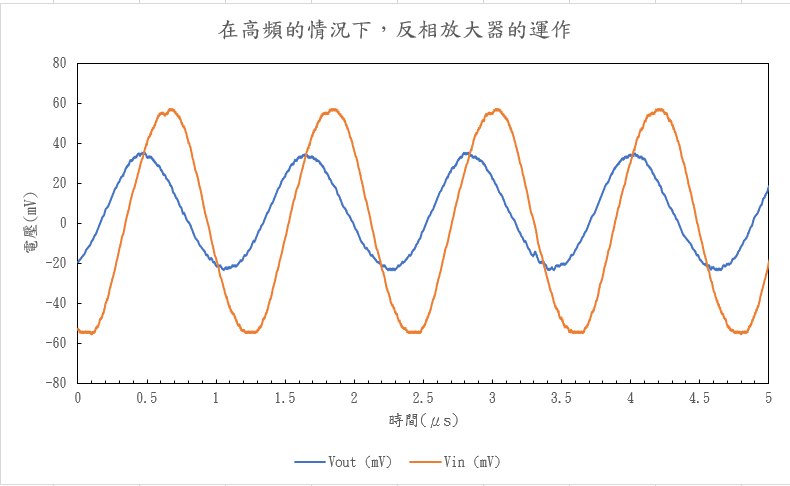
\includegraphics[width=0.45\linewidth]{figures/ia/Inverting amplifier_high freq.png}
    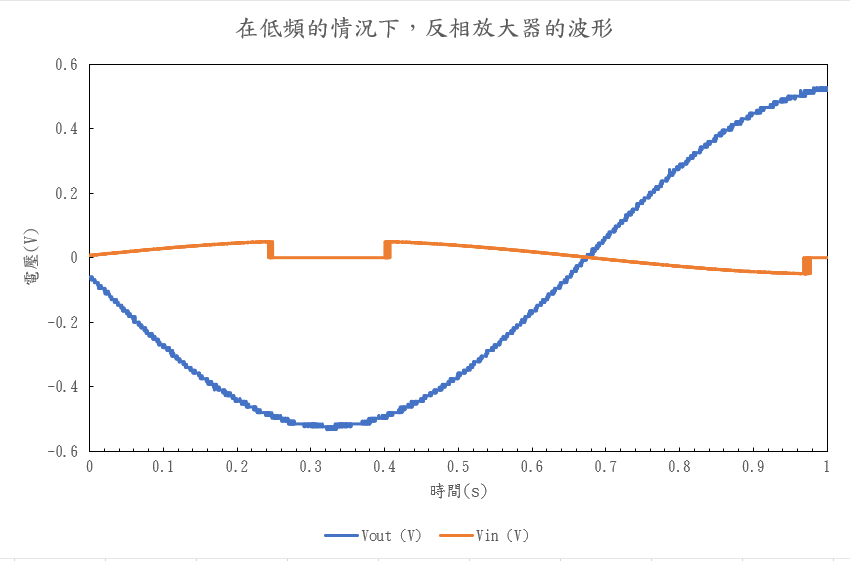
\includegraphics[width=0.45\linewidth]{figures/ia/Inverting amplifier_low freq.png}
    \caption{在高頻和低頻的情況下,反相放大器的運作情形}
    \label{fig:IA_freq.}
\end{figure}

高頻:$1MHz$之正弦波
\begin{itemize}
    \item 輸入振幅:$53.70mV$
    \item 輸出振幅:$109.5mV$
\end{itemize}

低頻:$1Hz$之正弦波
\begin{itemize}
    \item 輸入振幅:$1.029V$
    \item 輸出振幅:$--V$
\end{itemize}

% \clearpage

\noindent 分析:

從Fig.\ref{fig:IA_freq.}左圖可見在高頻的情況下,波形明顯失真,不但相位沒有差異$180^\circ$,增益也僅剩$\frac{110}{53.7}\approx 2.05$,與理論的$9.90$誤差為$79.3\%$,明顯的太小。

這可以歸咎於兩個原因:
\begin{enumerate}
    \item 頻率超過了增益-頻寬乘積$Gain-Bandwidth\ Product\ (GBW)$的限制:\\
    反相放大器的增益$A_v$與頻率的關係為
    \begin{equation}
        A_v(f) \times f=GBW
        \nonumber
    \end{equation}
    如果我們使用的放大器$GBW=1MHz$,而我們的輸入頻率達到$1MHz$,放大器可以維持的增益變成$A_v=\frac{1MHz}{1MHz}$,這就符合我們所看到的增益僅為約2倍的原因。
    \item 相位的延遲:\\放大器的輸出電壓變化速度有限,如果輸入的變化太快時會來不及反應,導致波形邊緣鈍化等失真。
\end{enumerate}

從Fig.\ref{fig:IA_freq.}右圖可見在低頻的情況下,波形有符合「相位差$180^\circ$」和「放大」這兩個特性,不過實驗數據無法測量輸出振幅,推測是因為輸出的振幅超過了示波器所能顯示的最大電壓,以至於無法偵測到。
    
    \item 試試看三角波輸入,這放大器是否非常"線性"?

\begin{figure}[h]
    \centering
    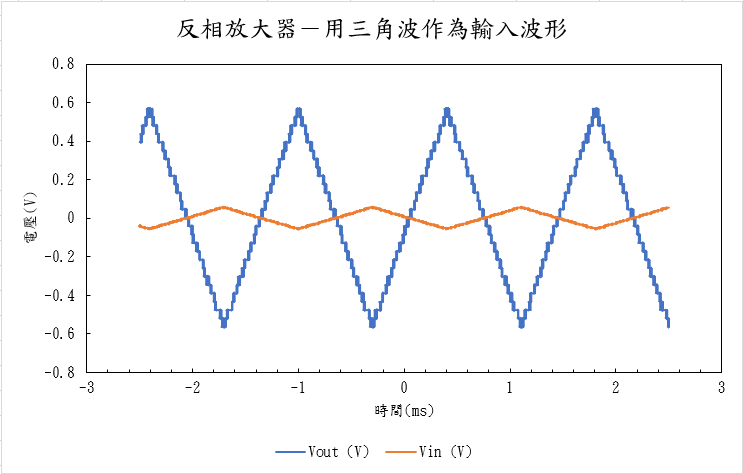
\includegraphics[width=0.7\linewidth]{figures/ia/Inverting amplifier with triangle wave input.png}
    \caption{反相放大器實驗中,將輸入訊號改成三角波後的情況}
    \label{fig:IA_tri}
\end{figure}

輸入振幅:$70.22mV$

輸出振幅:$697.2mV$

\noindent 分析:

我們的參數與第一步的初始設定一樣($V_{in}$為$1kHz$、$DC\ offset=0$、振幅為$0.1V$)但改成三角波輸入,而波形非常線性,是理想三角波的形狀。而計算出的增益為:$\frac{697}{70.2}\approx9.96$,與理論的$9.90$誤差為$0.6\%$,是理想的結果。
    
    \item 此放大器的輸入阻抗? 請先計算理論輸入阻抗(Hint: $Z=\frac{V}{I}$),再利用下圖等效電路圖,設計電路。試試不同的$ R_{test} $及$ V_s$,記錄$V_{out}$,推算出$R_{in}$。

    反相放大器的結構為:反相輸入端接一個電阻$R_1$,輸出端回接一個電阻$R_2$,而理想中的運算放大器有個特性:輸入端幾乎沒有電流流入,因此可以用簡單的模型簡化他;輸入阻抗為
    \begin{equation}
        Z_{in}=\frac{V_{in}}{I_{in}}
        \nonumber
    \end{equation}
而所有流入輸入端的電流都流過$R_1$,就可以得知:
\begin{equation}
    Z_{in}=R_1
    \nonumber
\end{equation}

在本次的實驗裡,$R_1=0.99k\Omega$,所以輸入阻抗為$0.99k\Omega$
    
\end{enumerate}



\subsection{誤差討論}

\noindent 本次可能造成誤差的原因:
\begin{enumerate}
    \item 在量測$R_1$、$R_2$時,可能因為三用電表有些許儀器誤差,導致不能量測到最精準的數值。
    \item 電子接線若過於老舊可能會造成訊號的雜訊,以及沒辦法完全在沒損耗能量的情況下傳遞訊號。
    \item 訊號產生器可能會造成些許的振幅偏差,造成理論值與實際值產生誤差。
\end{enumerate}



\section{非反相放大器}

\subsection{實驗步驟}
\begin{enumerate}
    \item 連接電路
    \item $V_{in}$ 用$1KHz$,$DC\ Offset=0$,振幅 $0.1Volt$之弦波輸入,測$V_{out}$,得出電壓增益。
    \item 將$V_{in}$之振幅加大,注意觀察$V_{out}$,$V_{out}$,的最大振幅為多少(不被削截)?
    \item 改變$V_{in}$的頻率,在很高或很低的頻率此放大器還正常工作嗎?
    \item 試試看三角波輸入,這放大器是否非常"線性"?
    \item 此放大器的輸入阻抗? 請先計算理論輸入阻抗(Hint: $Z=\frac{V}{I}$),再利用下圖等效電路圖,設計電路。試試不同的$ R_{test} $及$ V_s$,記錄$V_{out}$,推算出$R_{in}$;請觀察$ R_{test} $到多大時,$V_{out}$依舊沒有太多改變,由此判斷$ R_{in} $至少大於多少。
\end{enumerate}

\clearpage
\subsection{實驗分析}


\begin{enumerate}
    \item $V_{in}$ 用 1KHz,DC Offset=0,振幅 0.1Volt 之弦波輸入,測 $V_{out}$,得出電壓增益。實際使用:R1=0.99k$\Omega$、R2 = 9.80k$\Omega$
    
\begin{figure}[h]
    \centering
    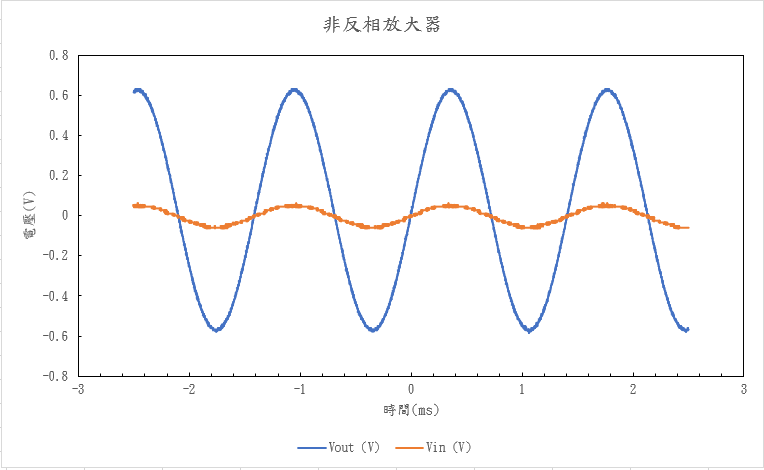
\includegraphics[width=0.7\linewidth]{figures/non-ia/non-inverting amplifier.png}
    \caption{經由非反相放大器的輸出波形與原訊號的比較}
    \label{fig:non_IA_normal}
\end{figure}

輸入振幅:$0.105V$

輸出振幅:$1.181V$

\noindent 分析:

因為非反相放大器的輸入接在運算放大器的非反相端(+),可以從上圖看出,輸出訊號與輸入訊號同相位。

\noindent 電壓增益計算:
根據增益計算的理論公式:
\begin{equation}
    A_v = 1+\frac{R_2}{R_1}
\end{equation}
帶入實際數值可得出理論增益約為10.90,而實測之增益值為$1.181/0.105 \approx 11.25$,誤差值$\approx3.2\%$,大致和理論值相符,顯示非反相放大器在穩態小訊號下具有穩定的增益效果。

\clearpage
\item 將 $V_{in}$ 之振幅加大,注意觀察 $V_{out}$ ,$V_{out}$ 的最大振幅為多少(不被削截)?
\begin{figure}[h]
    \centering
    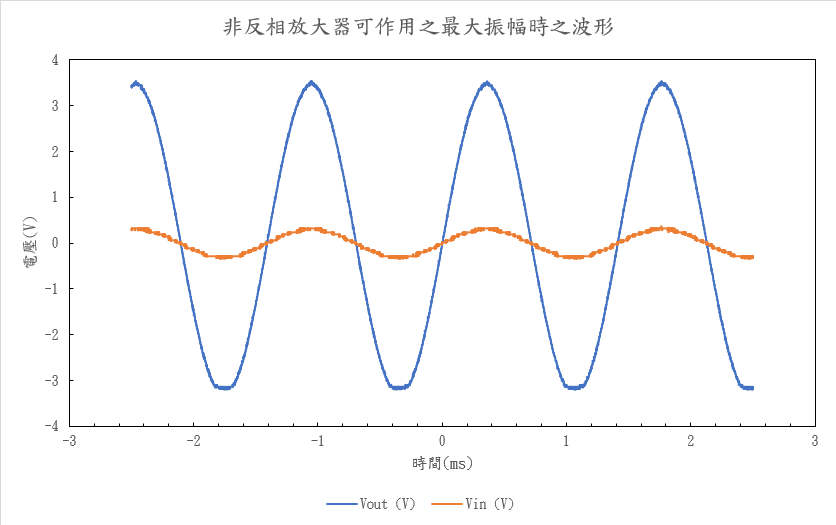
\includegraphics[width=0.7\linewidth]{figures/non-ia/non-inverting amplifier_max.png}
    \caption{非反相放大器可測量到的最大振幅}
    \label{fig:non_IA_Max}
\end{figure}

輸入振幅:$0.522V$

輸出振幅:$6.548V$

\noindent 分析:

當輸入達到 0.522V 時,可以觀察到輸出振幅達到約 6.548V時,波形開始產生clipping的現象,表示放大器的輸出已接近電源供應(±5V)的限制範圍。而因為非反相放大器的輸入訊號是接在( +) 端,輸出與輸入相位相同,因此當輸入電壓往正方向增加時,輸出也朝正方向放大。所以當輸出電壓超過放大器所能提供的最大正電壓,波形就會被「截斷」,造成削波。而如果輸入朝負方向增加,輸出也會朝負方向增加,超出範圍時同樣也會產生對稱的削波。

\noindent 電壓增益計算:實際增益值為$6.548/0.522\approx12.54$
誤差約為$15\%$,推測誤差值較大的是由於我們須以肉眼辨識波行產生clipping現象與否,且輸入振幅是以旋鈕方式調節,會讓實驗結果沒那麼精確,導致的人為誤差對結果有較大影響。


% \clearpage



% \clearpage


\item 改變 $V_{in}$ 的頻率,在很高或很低的頻率此放大器還正常工作嗎?
\begin{figure}[h]
    \centering
    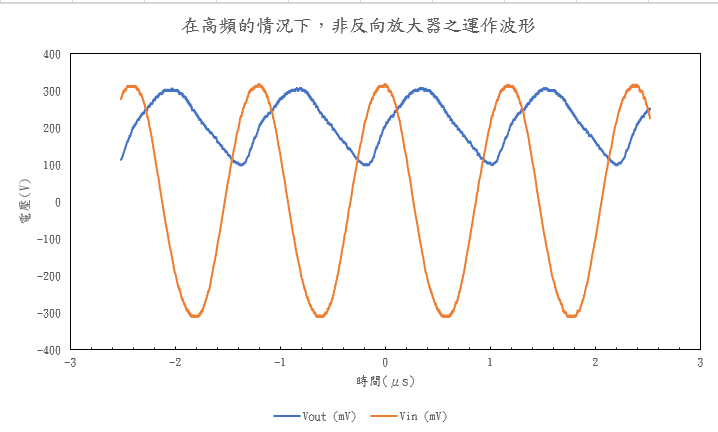
\includegraphics[width=0.45\linewidth]{figures/non-ia/non-inverting amplifier_high freq.png}
    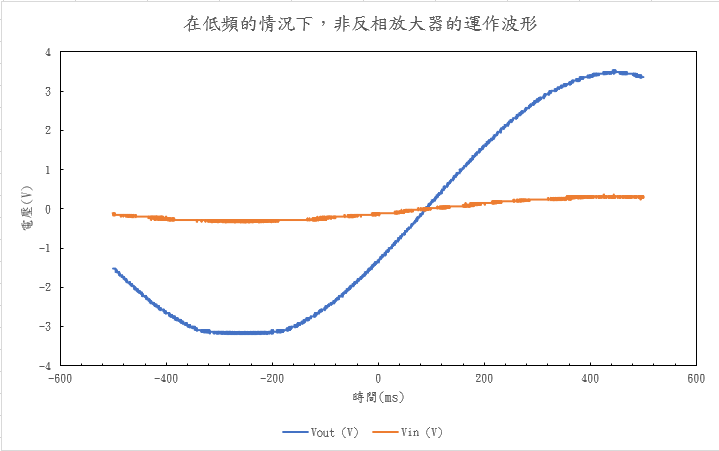
\includegraphics[width=0.45\linewidth]{figures/non-ia/non-inverting amplifier_low freq.png}
    \caption{在高頻和低頻的情況下,反相放大器的運作情形}
    \label{fig:non_IA_freq}
\end{figure}
\clearpage
高頻:$1MHz$之正弦波
\begin{itemize}
    \item 輸入振幅:$201.6mV$
    \item 輸出振幅:$616.2mV$
\end{itemize}

低頻:$1Hz$之正弦波
\begin{itemize}
    \item 輸入振幅:$0.609V$
    \item 輸出振幅:$6.558V$
\end{itemize}

\noindent 分析:

從兩組實驗結果皆可得知,在高頻時輸出波形明顯受到失真影響;而在低頻時,放大效果維持良好,波形穩定。正弦波在高頻(1 MHz)下之實測增益為3.06,誤差為71.9\%;三角波在高頻(1 MHz)下之實測增益為1.85,誤差為83.03\%,此外,波形也出現邊緣模糊、相位延遲等現象。

這類效應的產生,主要可歸因於:
\begin{itemize}
    \item \textbf{GBW限制:}UA741 的 GBW 約為 1 MHz,當輸入頻率接近該極限時,放大器所能維持的增益將下降。根據公式:
    \begin{equation}
        A_v(f)\times f = GBW
    \end{equation}
    當 f = 1 MHz 時,理論上最大增益應降至 1,因此我們實測得到的增益數值其實已經超過預期,推測是部分測量或器件提供了額外增益導致的。
    \item \textbf{放大器反應速度有限:}當訊號變化過快(也就是高頻)時,放大器的輸出跟不上輸入電壓的變化速度,導致波形出現變形、邊緣變鈍的現象。
\end{itemize}

\begin{figure}[h]
    \centering
    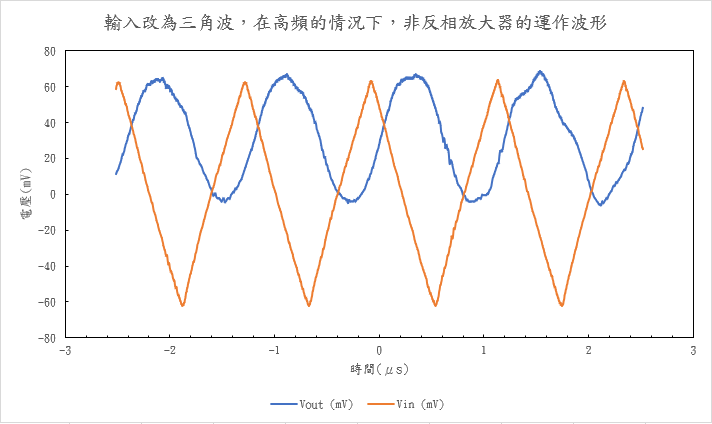
\includegraphics[width=0.45\linewidth]{figures/non-ia/non-inverting amplifier_tri_high freq.png}
    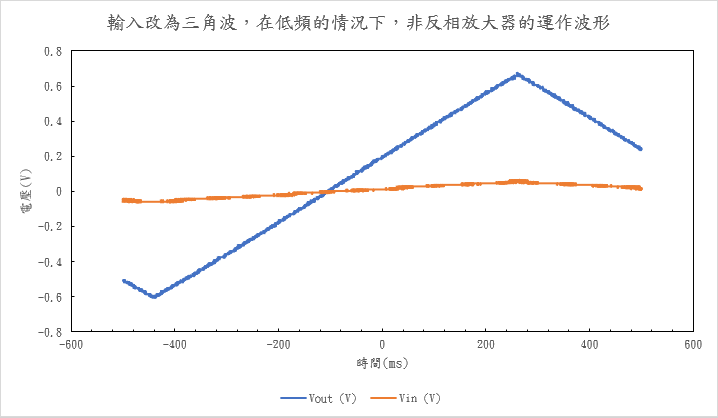
\includegraphics[width=0.45\linewidth]{figures/non-ia/non-inverting amplifier_tri_low freq.png}
    \caption{將輸入改為三角波,在高頻和低頻的情況下,反相放大器的運作情形}
    \label{fig:non_IA_tri_freq}
\end{figure}

高頻:$1MHz$之三角波
\begin{itemize}
    \item 輸入振幅:$121.9mV$
    \item 輸出振幅:$65.79mV$
\end{itemize}

低頻:$1Hz$之三角波
\begin{itemize}
    \item 輸入振幅:$0.105V$
    \item 輸出振幅:$1.157V$
\end{itemize}


\item 試試看三角波輸入,這放大器是否非常「線性」?

\begin{figure}[h]
    \centering
    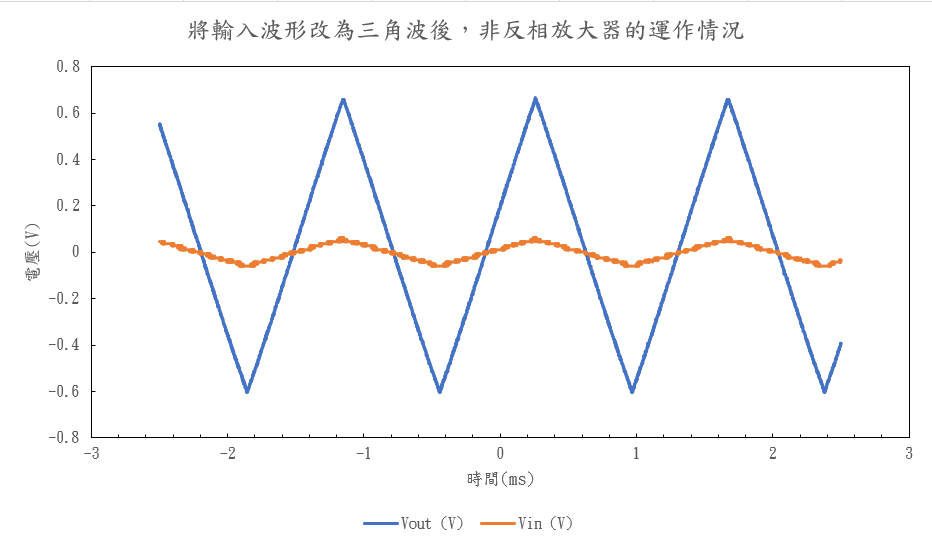
\includegraphics[width=0.7\linewidth]{figures/non-ia/non-inverting amplifier_tri.png}
    \caption{非反相放大器實驗中,將輸入訊號改成三角波後的情況}
    \label{fig:non_IA_tri}
\end{figure}

輸入振幅:$0.070V$

輸出振幅:$0.912V$

\noindent 分析:

輸出波形與輸入的三角波形狀高度相符,無明顯變形或扭曲,可看出放大器的輸出在此輸入振幅下仍具有良好的線性。增益值為0.912/0.070=13.03,誤差約為19.5\%,雖然誤差數值偏高,但波型看起來符合理想,誤差來源可能是pico截取振幅時對尖角取樣的精度問題。

\item 此放大器的輸入阻抗? 請先計算理論輸入阻抗(Hint: Z=V/I),再利用下圖等效電路圖,設計電路。試試不同的 $R_{test}$ 及 Vs,記錄 $V_{out}$,推算出 Rin\\
非反相放大器輸入接在 + 端,特性是+ 端沒有任何電阻與回授直接連接,因此阻抗主要由運算放大器本身的輸入阻抗決定(理想情況下為無限大)。由於理想運算放大器具備無窮大的輸入阻抗,實際上電流流入 + 端極微小。因此若在輸入端串接一個外部電阻 $R_{test}$,就只有在$R_{test}$ 明顯小於輸入阻抗時,才會觀察到明顯的輸出電壓衰減 。

根據電路模型推倒可得:
\begin{equation}
    V_{out}=\frac{A_vR_{in}}{R_{test}+R_{in}}V_s
\end{equation}
可改寫出
\begin{equation}
    R_{in}=\frac{R_{test}V_{out}}{A_vV_s-V_{out}}
\end{equation}
帶入實驗測得之實際數值:
\begin{itemize}
    \item $R_{test}=9.86k\Omega$,$R_1= 470 \Omega$,$R_2=1k \Omega$,$V_{in}=109.8mV$,$V_{out}=333.7 mV$,可得$R_{in}$之值為337k$\Omega$
    \item $R_{test}=480 \Omega$,$R_1= 470 \Omega$,$R_2=1k \Omega$,$V_{in}=109.9mV$,$V_{out}=328.9 mV$,可得$R_{in}$之值為11k$\Omega$
\end{itemize}
當 $R_{test}$ 很大(9.86k$\Omega$)時,$R_{in} $推得很高;但當 $R_{test}$ 跟 Rin 在同量級時,反推出 Rin 值會明顯下降。

\item 關於第 5 項,請觀察 $R_{test}$ 到多大時,$V_{out} $依舊沒有太多改變,由此判斷$ R_{in}$ 至少大於多少。\\
根據實驗觀察,當 $R_{test}$ 增加至 100k$\Omega$ 時,$V_{out}$ 變化仍不顯著,因此可推論此非反相放大器之輸入阻抗 $R_{in }$至少大於 100k$\Omega$,符合理論上非反相輸入具有高阻抗的預期。

\end{enumerate}

\subsection{誤差討論}

\noindent 本次可能造成誤差的原因:
\begin{enumerate}
    \item 在量測$R_1$、$R_2$時,可能因為三用電表有些許儀器誤差,導致不能量測到最精準的數值。
    \item 電子接線若過於老舊可能會造成訊號的雜訊,以及沒辦法完全在沒損耗能量的情況下傳遞訊號。
    \item 訊號產生器可能會造成些許的振幅偏差,造成理論值與實際值產生誤差。
\end{enumerate}


% \clearpage
\section{隨耦器}
\subsection{實驗步驟}
\begin{enumerate}
    \item 連接電路
    \item $V_{in}$ 用$1KHz$,$DC\ Offset=0$,振幅 $0.1Volt$之弦波輸入,測$V_{out}$,得出電壓增益。
    \item 將$V_{in}$之振幅加大,注意觀察$V_{out}$,$V_{out}$,的最大振幅為多少(不被削截)?
    \item 改變$V_{in}$的頻率,在很高或很低的頻率此放大器還正常工作嗎?
    \item 試試看三角波輸入,這放大器是否非常"線性"?
    %\item 此放大器的輸入阻抗? 請先計算理論輸入阻抗(Hint: $Z=\frac{V}{I}$),再利用下圖等效電路圖,設計電路。試試不同的$ R_{test} $及$ V_s$,記錄$V_{out}$,推算出$R_{in}$;請觀察$ R_{test} $到多大時,$V_{out}$依舊沒有太多改變,由此判斷$ R_{in} $至少大於多少。
\end{enumerate}

\clearpage
\subsection{實驗分析}

\begin{enumerate}
    \item $V_{in}$ 用 1KHz,DC Offset=0,振幅 0.1Volt 之弦波輸入,測 $V_{out}$,得出電壓增益。


\begin{figure}[h]
    \centering
    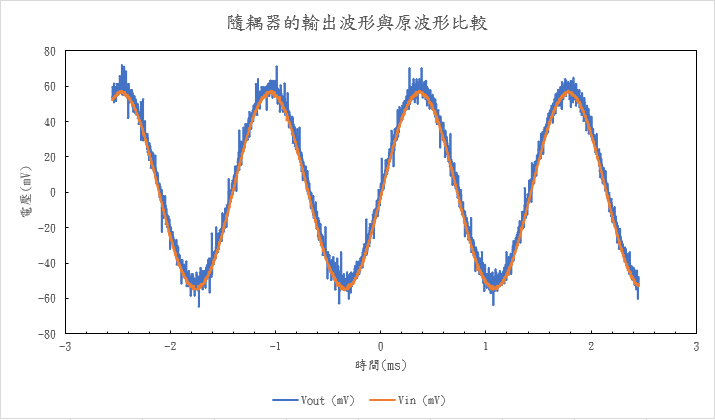
\includegraphics[width=0.7\linewidth]{figures/Buffer amplifier/Buffer amplifier.png}
    \caption{經由隨耦器的輸出波形與原訊號的比較}
    \label{fig:BA_normal}
\end{figure}

輸入振幅:$109.8mV$

輸出振幅:$107.4mV$

\noindent 分析:

由Fig.\ref{fig:BA_normal}可觀察,隨耦器的增益為1,且輸出相位與輸入相位相同,使得輸入與輸出訊號重合,此性質符合預期。

\item 將 $V_{in}$ 之振幅加大,注意觀察 $V_{out}$ ,$V_{out}$ 的最大振幅為多少(不被削截)?
\begin{figure}[h]
    \centering
    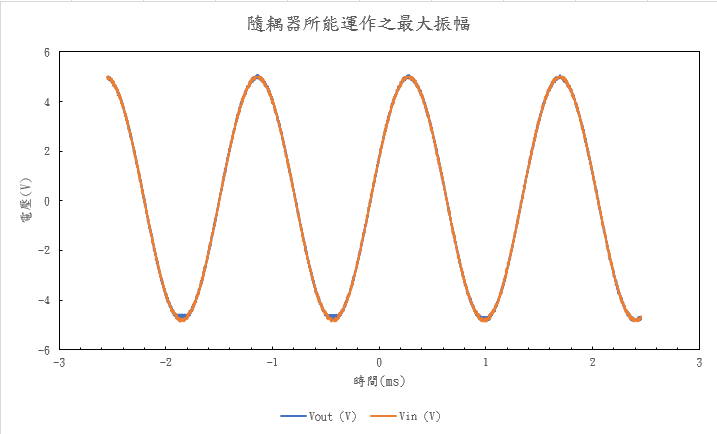
\includegraphics[width=0.7\linewidth]{figures/Buffer amplifier/Buffer amplifier_max.png}
    \caption{隨耦器可測量到的最大振幅}
    \label{fig:BA_Max}
\end{figure}

輸入振幅:$9.634V$

輸出振幅:$9.555V$

\noindent 分析:

當輸入達到 9.632V 時,可以觀察到輸出振幅達到約 9.555V時,波形開始產生clipping的現象,表示隨耦器的輸出已接近電源供應的限制範圍。而因為隨耦器的輸入訊號是接在(+) 端,輸出與輸入相位相同,因此當輸入電壓往正方向增加時,輸出也朝正方向放大。所以當輸出電壓超過放大器所能提供的最大正電壓,波形就會被「截斷」,造成削波。而如果輸入朝負方向增加,輸出也會朝負方向增加,超出範圍時同樣也會產生對稱的削波。


\item 改變 $V_{in}$ 的頻率,在很高或很低的頻率此放大器還正常工作嗎?

% \clearpage
\begin{figure}[h]
    \centering
    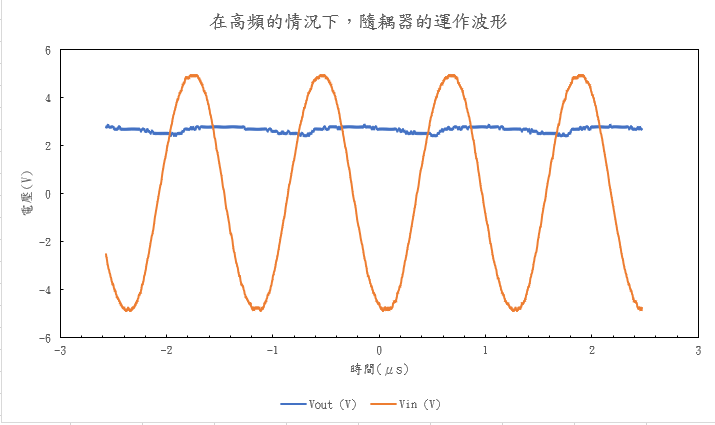
\includegraphics[width=0.45\linewidth]{figures/Buffer amplifier/Buffer amplifier_high freq.png}
    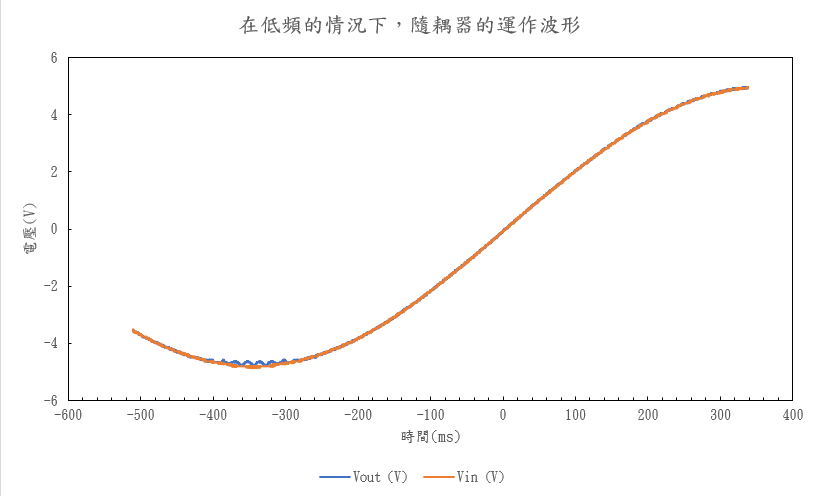
\includegraphics[width=0.45\linewidth]{figures/Buffer amplifier/Buffer amplifier_low freq.png}
    \caption{在高頻和低頻的情況下,隨耦器的運作情形}
    \label{fig:BA_freq}
\end{figure}

高頻:$1MHz$之正弦波
\begin{itemize}
    \item 輸入振幅:$9.589V$
    \item 輸出振幅:$0.260V$
\end{itemize}

低頻:$1Hz$之正弦波
\begin{itemize}
    \item 輸入振幅:$--V$
    \item 輸出振幅:$--V$
\end{itemize}


\noindent
從Fig.\ref{fig:BA_freq}左圖發現,隨耦器在高頻的情況下,輸出訊號出現不尋常的狀況,如:沒有震盪,不過在低頻下(Fig.\ref{fig:BA_freq}右圖),不尋常的狀況就沒有出現,因此推測此隨耦器無法正常在高頻下的運作。


\begin{figure}[h]
    \centering
    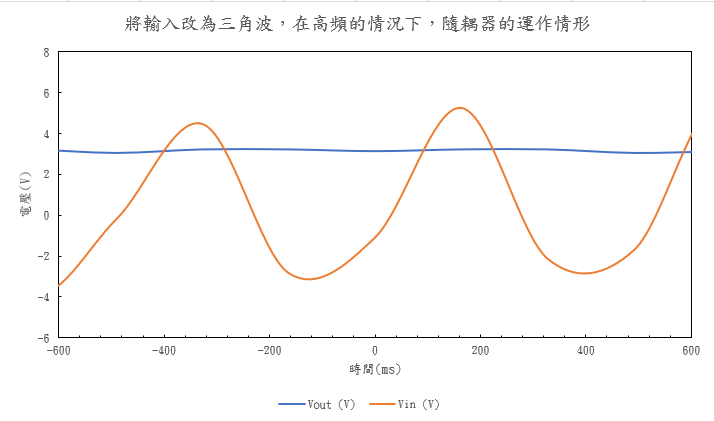
\includegraphics[width=0.45\linewidth]{figures/Buffer amplifier/Buffer amplifier_tri_high freq.png}
    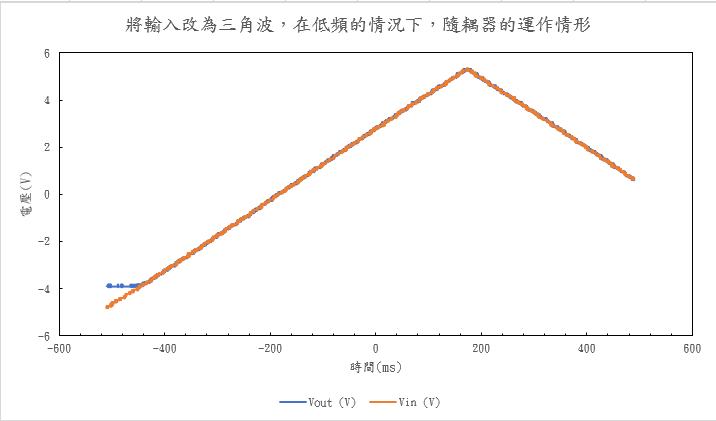
\includegraphics[width=0.45\linewidth]{figures/Buffer amplifier/Buffer amplifier_tri_low freq.png}
    \caption{將輸入改為三角波,在高頻和低頻的情況下,反相放大器的運作情形}
    \label{fig:BA_tri_freq}
\end{figure}

高頻:$1MHz$之三角波
\begin{itemize}
    \item 輸入振幅:$10.71V$
    \item 輸出振幅:$0.261V$
\end{itemize}

低頻:$1Hz$之三角波
\begin{itemize}
    \item 輸入振幅:$6.709V$
    \item 輸出振幅:$8.193V$
\end{itemize}

\noindent 分析:

從Fig.\ref{fig:BA_tri_freq}左圖發現,隨耦器在高頻的情況下,輸出訊號出現不尋常的狀況,如:沒有震盪,不過在低頻下(Fig.\ref{fig:BA_tri_freq}右圖),不尋常的狀況就沒有出現。此現象與正弦波相同,因此推測此隨耦器無法正常在高頻下的運作。


% \clearpage
\item 試試看三角波輸入,這放大器是否非常「線性」?
\begin{figure}[h]
    \centering
    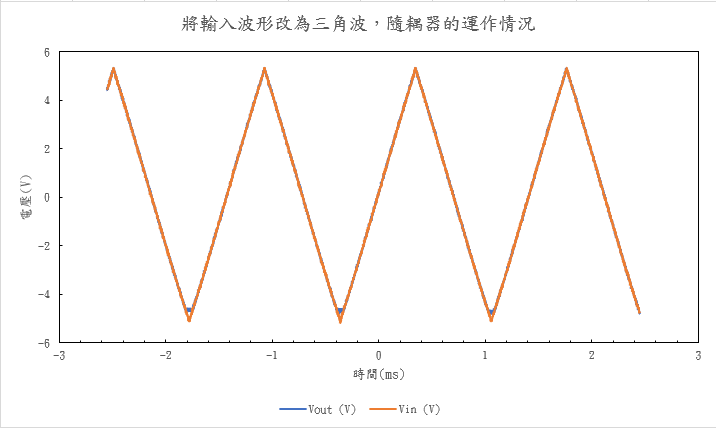
\includegraphics[width=0.7\linewidth]{figures/Buffer amplifier/Buffer amplifier_tri.png}
    \caption{隨耦器實驗中,將輸入訊號改成三角波後的情況}
    \label{fig:BA_tri}
\end{figure}

輸入振幅:$8.904V$

輸出振幅:$9.504V$


\noindent 分析:

輸出波形與輸入的三角波形狀高度相符,無明顯變形或扭曲,可看出放大器的輸出在此輸入振幅下仍具有良好的線性


\end{enumerate}

% \clearpage

\section{問題與討論}
\hfill

將練習1和2中所得之增益和在預習問題2中所求得的理論值比較。不一樣的可能原因?

\subsection{練習一:反相放大器}
\begin{itemize}
    \item 理論增益:
    \begin{equation}
        A_v=-\frac{R_2}{R_1}=-\frac{9.80k\Omega}{0.99k\Omega}\approx -9.90
        \nonumber
    \end{equation}
    \item 實驗測得增益:
    \begin{itemize}
        \item 小訊號:$\frac{1.043}{0.088} \approx 11.9$,誤差約+20.2\%
        \item 最大振幅:$\frac{5.879}{0.608} \approx 9.64$,誤差約-2.6\%
        \item 三角波:$\frac{697.2}{70.22} \approx 9.96$,誤差約+0.6\%
        \item 高頻:$\frac{109.5}{53.70} \approx 2.04$,誤差約-79.4\%
    \end{itemize}
\end{itemize}

\subsection{練習二:非反相放大器}
\begin{itemize}
    \item 理論增益:
    \begin{equation}
        A_v=1+\frac{R_2}{R_1}=1+\frac{9.80k\Omega}{0.99k\Omega}=1+9.90=10.90
        \nonumber
    \end{equation}
    \item 實驗測得增益:
    \begin{itemize}
        \item 小訊號:$\frac{1.181}{0.105} \approx 11.25$,誤差約+3.2\%
        \item 最大振幅:$\frac{6.548}{0.522} \approx 12.54$,誤差約+15.0\%
        \item 三角波:$\frac{0.912}{0.070} \approx 13.03$,誤差約+19.5\%
        \item 高頻:$\frac{616.2}{201.6} \approx 3.06$,誤差約-71.9\%
    \end{itemize}
\end{itemize}

\subsection{分析不一樣的原因}
\hfill

\begin{enumerate}
    \item 小訊號產生誤差的可能原因:
    \begin{itemize}
        \item 波形判讀誤差:如果輸入訊號很小,微小的數值差距就會導致計算增益時造成就大的誤差。
        \item 訊號源的內阻或雜訊:輸入訊號可能本身就有非零輸出阻抗或背景雜訊,使$V_{in}$在進到放大器前就有些許失真。
        \item 在電流傳輸的過程可能會有點能量損耗,導致放大效果有誤差。
    \end{itemize}
    \item 高頻誤差非常大的原因:
    \begin{itemize}
        \item 頻率超過$GBW$限制:UA741的典型增益-頻寬乘積(GBW)只有約$1MHz$,在1MHz操作下,最大理論增益是 $1$,而不是理論設計的$9.90$或$10.90$。
        \item 相位延遲和波形失真:高頻下放大器反應不及,導致訊號變形和相位失真。
    \end{itemize}
\end{enumerate}

更多誤差討論可見我們在各種放大器之運用的數據分析後的誤差分析。


%練習一不是不用做嗎幹


\section{總結}
\hfill

本次實驗旨在探討運算放大器 UA741 在三種基本應用下的行為與特性:反相放大器、非反相放大器與隨耦器(電壓跟隨器)。透過麵包板實作與示波器觀測,我們分析了不同輸入條件(頻率、振幅、波形)對輸出訊號的影響。結果顯示三種電路在低頻、小訊號下表現良好,增益接近理論值,具備預期的相位關係與線性響應。然而在高頻或大振幅下,尤其超出增益-頻寬乘積(GBW)範圍時,輸出波形會出現削截、相位延遲與失真現象,反映出實際元件的限制。誤差分析指出,儀器誤差、老舊接線與訊號源穩定性皆可能影響實驗準確性。整體而言,實驗成功驗證了運算放大器基本應用的理論模型,也讓我們對實際操作中的限制有更深刻理解。


\section{分工內容}
\begin{itemize}
    \item 洪瑜:反向放大器
    \item 黃巧涵:非反向放大器
    \item 洪懌平:隨耦器
\end{itemize}

\section{參考文獻}
\hfill
\begin{enumerate}
    \item \url{https://shorturl.at/kj0ru}
\end{enumerate}


\end{CJK}
\end{document}
